\subsection{Verification of Rates of Convergence}
In this subsection we verify the theoretical error estimates developed in
\autoref{sec:QGEError}. To this end, we apply the Argyris FE in space while
applying implicit Euler in time to \eqref{eqn:QGE_psi}. To solve the resulting
nonlinear system at each time step we apply Newton's method where the Newton's
method is considered to have converged when the $L^2$-norm of the difference in
the current Newton iterate and the previous Newton iterate is less than
$10^{-7}$. Additionally, in each of the following computational tests we take
$Re = 1$, $Ro = 1$, and $h = \nicefrac{1}{20}$ unless otherwise stated.

\subsubsection*{Test 1}
For this test we take the exact solution to be
\begin{equation}
  \psi(t;x,y) = \left(\sin \pi x \sin \pi y\right)^2 \sin t
  \label{eqn:Test1}
\end{equation}
which is very similar to \textbf{Test 6} in \cite{Foster}. Here we add the time
dependence in the sine term and let $\Omega = [0,1]^2$. The time interval for
integration is $t = [0,\frac{\pi}{2}]$. This test will have an intensifying
western boundary layer as time increases.

\begin{table}
  \begin{center}
    \begin{tabular}{|c|c|c|c|c|}
      \hline
      $k$ & $h$ & DoFs & $e_{L^2}$ & $L^2$ order \\% & $e_{H^1}$ & $H^1$ order & $e_{H^2}$ & $H^2$ order \\
      \hline
      $\nicefrac{1}{2}$ & $\nicefrac{1}{16}$ & $2853$ & $5.65\times 10^{-4}$ & $-$ \\%& $0.00293$ & $-$ & $0.01971$ & $-$ \\
      $\nicefrac{1}{4}$ & $\nicefrac{1}{16}$ & $2853$ & $3.49\times 10^{-4}$ & $0.697$ \\%& $0.001807$ & $0.6971$ & $0.01216$ & $0.697$ \\
      $\nicefrac{1}{8}$ & $\nicefrac{1}{16}$ & $2853$ & $1.916\times 10^{-4}$ & $0.864$ \\%& $0.0009931$ & $0.8636$ & $0.006683$ & $0.8634$ \\
      $\nicefrac{1}{16}$ & $\nicefrac{1}{16}$ & $2853$ & $1.001\times 10^{-4}$ & $0.937$ \\%& $0.0005189$ & $0.9366$ & $0.003494$ & $0.9359$ \\
      $\nicefrac{1}{32}$ & $\nicefrac{1}{16}$ & $2853$ & $5.11\times 10^{-5}$ & $0.970$ \\%& $0.000265$ & $0.9696$ & $0.001787$ & $0.9668$ \\
      $\nicefrac{1}{64}$ & $\nicefrac{1}{16}$ & $2853$ & $2.58\times 10^{-5}$ & $0.985$ \\%& $0.0001339$ & $0.9851$ & $0.0009098$ & $0.9743$ \\
      $\nicefrac{1}{128}$ & $\nicefrac{1}{16}$ & $2853$ & $1.30\times 10^{-5}$ & $0.993$ \\%& $6.728\times 10^{-5}$ & $0.9925$ & $0.0004705$ & $0.9513$ \\
      $\nicefrac{1}{256}$ & $\nicefrac{1}{16}$ & $2853$ & $6.51\times 10^{-6}$ & $0.996$ \\%& $3.374\times 10^{-5}$ & $0.9959$ & $0.0002607$ & $0.8516$ \\
      $\nicefrac{1}{512}$ & $\nicefrac{1}{16}$ & $2853$ & $3.26\times 10^{-6}$ & $0.998$ \\%& $1.691\times 10^{-5}$ & $0.9965$ & $0.0001715$ & $0.6046$ \\
      $\nicefrac{1}{1024}$ & $\nicefrac{1}{16}$ & $2853$ & $1.63\times 10^{-6}$ & $0.999$ \\%& $8.497\times 10^{-6}$ & $0.9927$ & $0.0001405$ & $0.2878$ \\
      \hline

    \end{tabular}
  \end{center}
  \caption{Observed order of convergence for Implicit-Euler applied to
    \eqref{eqn:QGE_psi} with the exact solution \eqref{eqn:Test1}.
    %Note the observed order of convergence matches the theoretical error estimates developed in \autoref{sec:QGEError}.
  }
  \label{tab:Test1Time}
\end{table}

\begin{figure}
  \begin{center}
    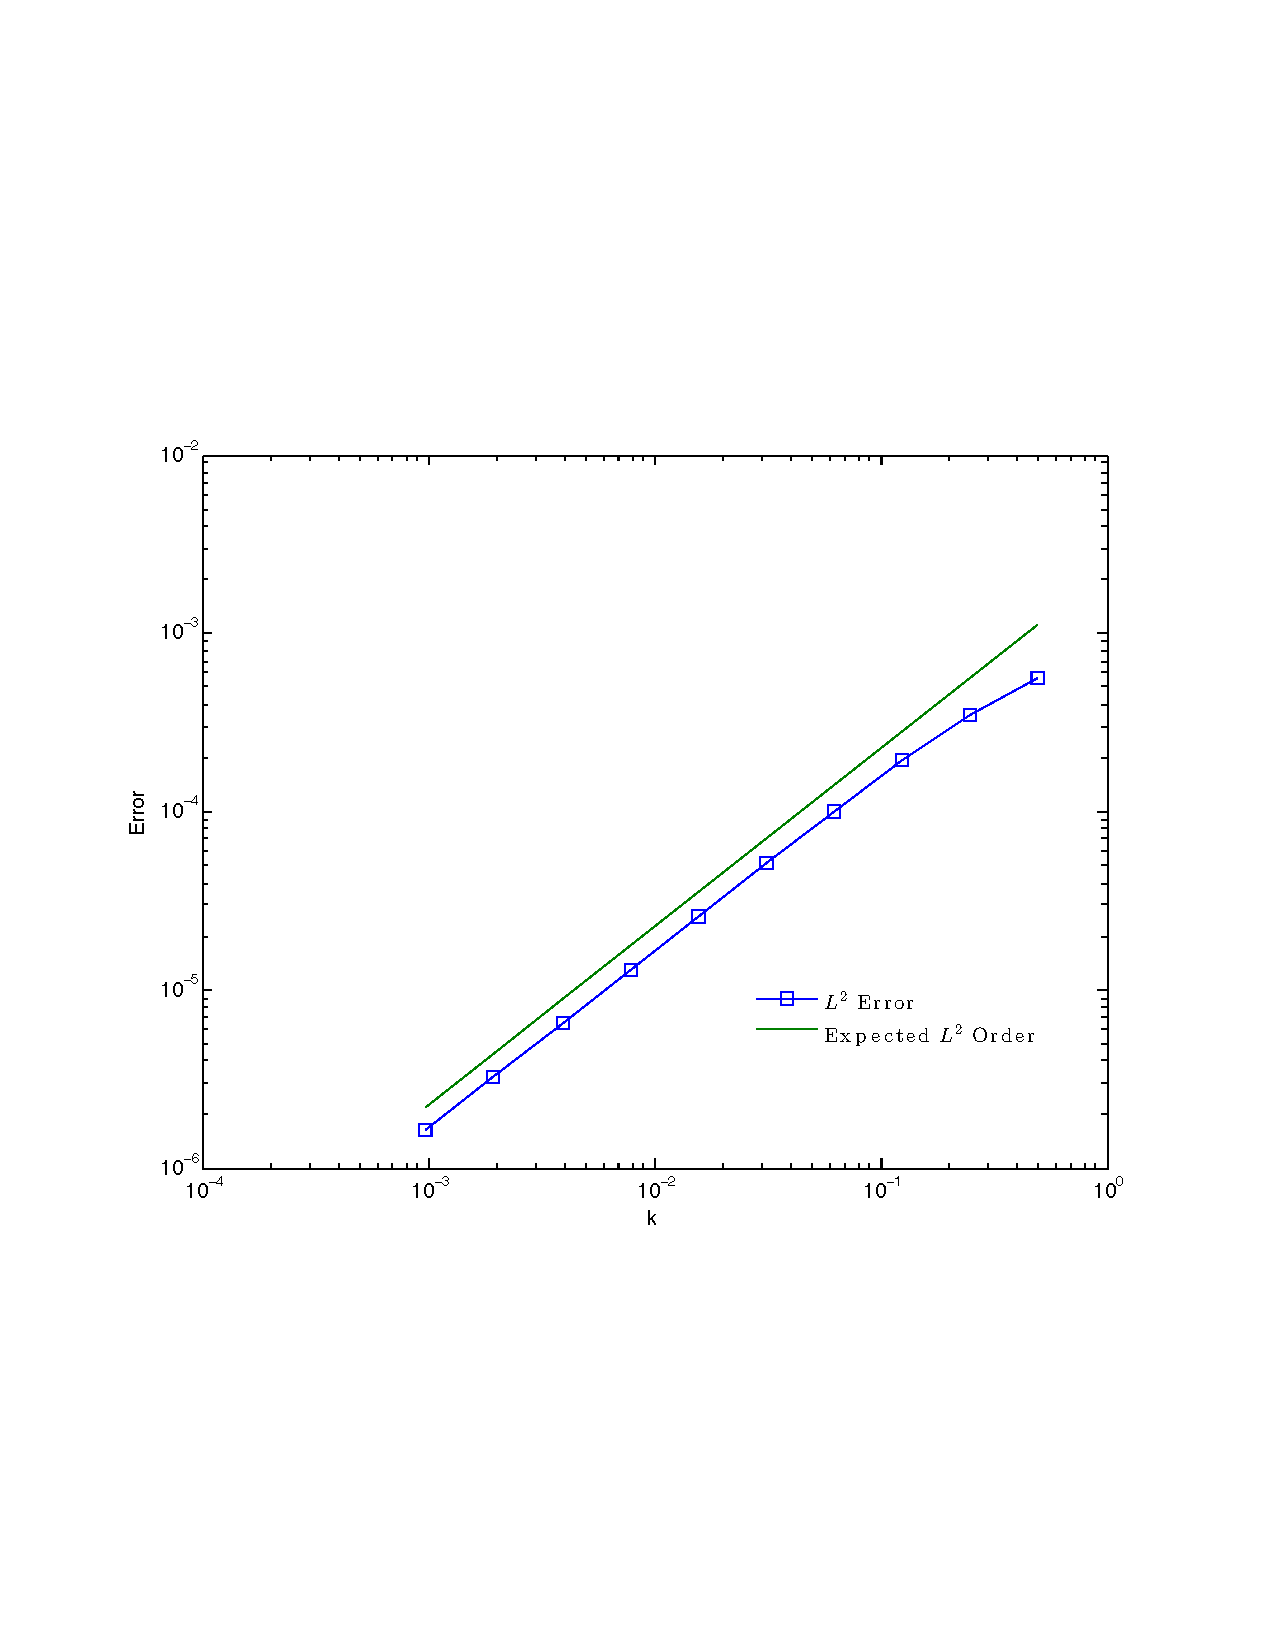
\includegraphics[scale=0.6]{sin2sin2sinTimeConvergence.pdf}
    \caption{Observed order of convergence for Implicit-Euler applied to
      \eqref{eqn:QGE_psi} with the exact solution \eqref{eqn:Test1}.}
  \label{fig:Test1Time}
  \end{center}
\end{figure}

\begin{table}
  \begin{center}
    \begin{tabular}{|c|c|c|c|c|c|c|c|c|}
      \hline
      $k$ & $h$ & DoFs & $e_{L^2}$ & $L^2$ order & $e_{H^1}$ & $H^1$ order & $e_{H^2}$ & $H^2$ order \\
      \hline
      $\nicefrac{1}{8192}$ & $\nicefrac{1}{2}$ & $38$ & $1.23\times 10^{-2}$ & $-$ & $1.18\times 10^{-1}$ & $-$ & $1.57\times 10^0$ & $-$ \\
      $\nicefrac{1}{8192}$ & $\nicefrac{1}{4}$ & $174$ & $2.12\times 10^{-5}$ & $9.18$ & $7.31\times 10^{-4}$ & $7.34$ & $2.79\times 10^{-2}$ & $5.81$ \\
      $\nicefrac{1}{8192}$ & $\nicefrac{1}{8}$ & $662$ & $7.88\times 10^{-7}$ & $4.75$ & $4.59\times 10^{-5}$ & $3.99$ & $3.04\times 10^{-3}$ & $3.20$ \\
      $\nicefrac{1}{8192}$ & $\nicefrac{1}{16}$ & $2853$ & $7.87\times 10^{-9}$ & $6.65$ & $9.05\times 10^{-7}$ & $5.67$ & $1.29\times 10^{-4}$ & $4.56$ \\
      $\nicefrac{1}{8192}$ & $\nicefrac{1}{32}$ & $11690$ & $6.97\times 10^{-11}$ & $6.82$ & $1.88\times 10^{-8}$ & $5.59$ & $5.98\times 10^{-6}$ & $4.43$ \\
      $\nicefrac{1}{8192}$ & $\nicefrac{1}{64}$ & $47958$ & $7.23\times 10^{-12}$ & $3.27$ & $5.26\times 10^{-10}$ & $5.16$ & $3.43\times 10^{-7}$ & $4.12$ \\
      \hline
    \end{tabular}
  \end{center}
  \caption{Observed spatial orders of convergence for Argyris applied to
    \eqref{eqn:QGE_psi} with the exact solution \eqref{eqn:Test2} using implicit
    Euler for time discretization. Note the observed orders of convergence
    nearly matches the theoretical error estimates developed in
    \autoref{sec:QGEError}. The $L^2$ order, however, drops off for the last
    spatial discretization due to nearing the machine epsilon.}
  \label{tab:Test1Space}
\end{table}

\begin{figure}
  \begin{center}
    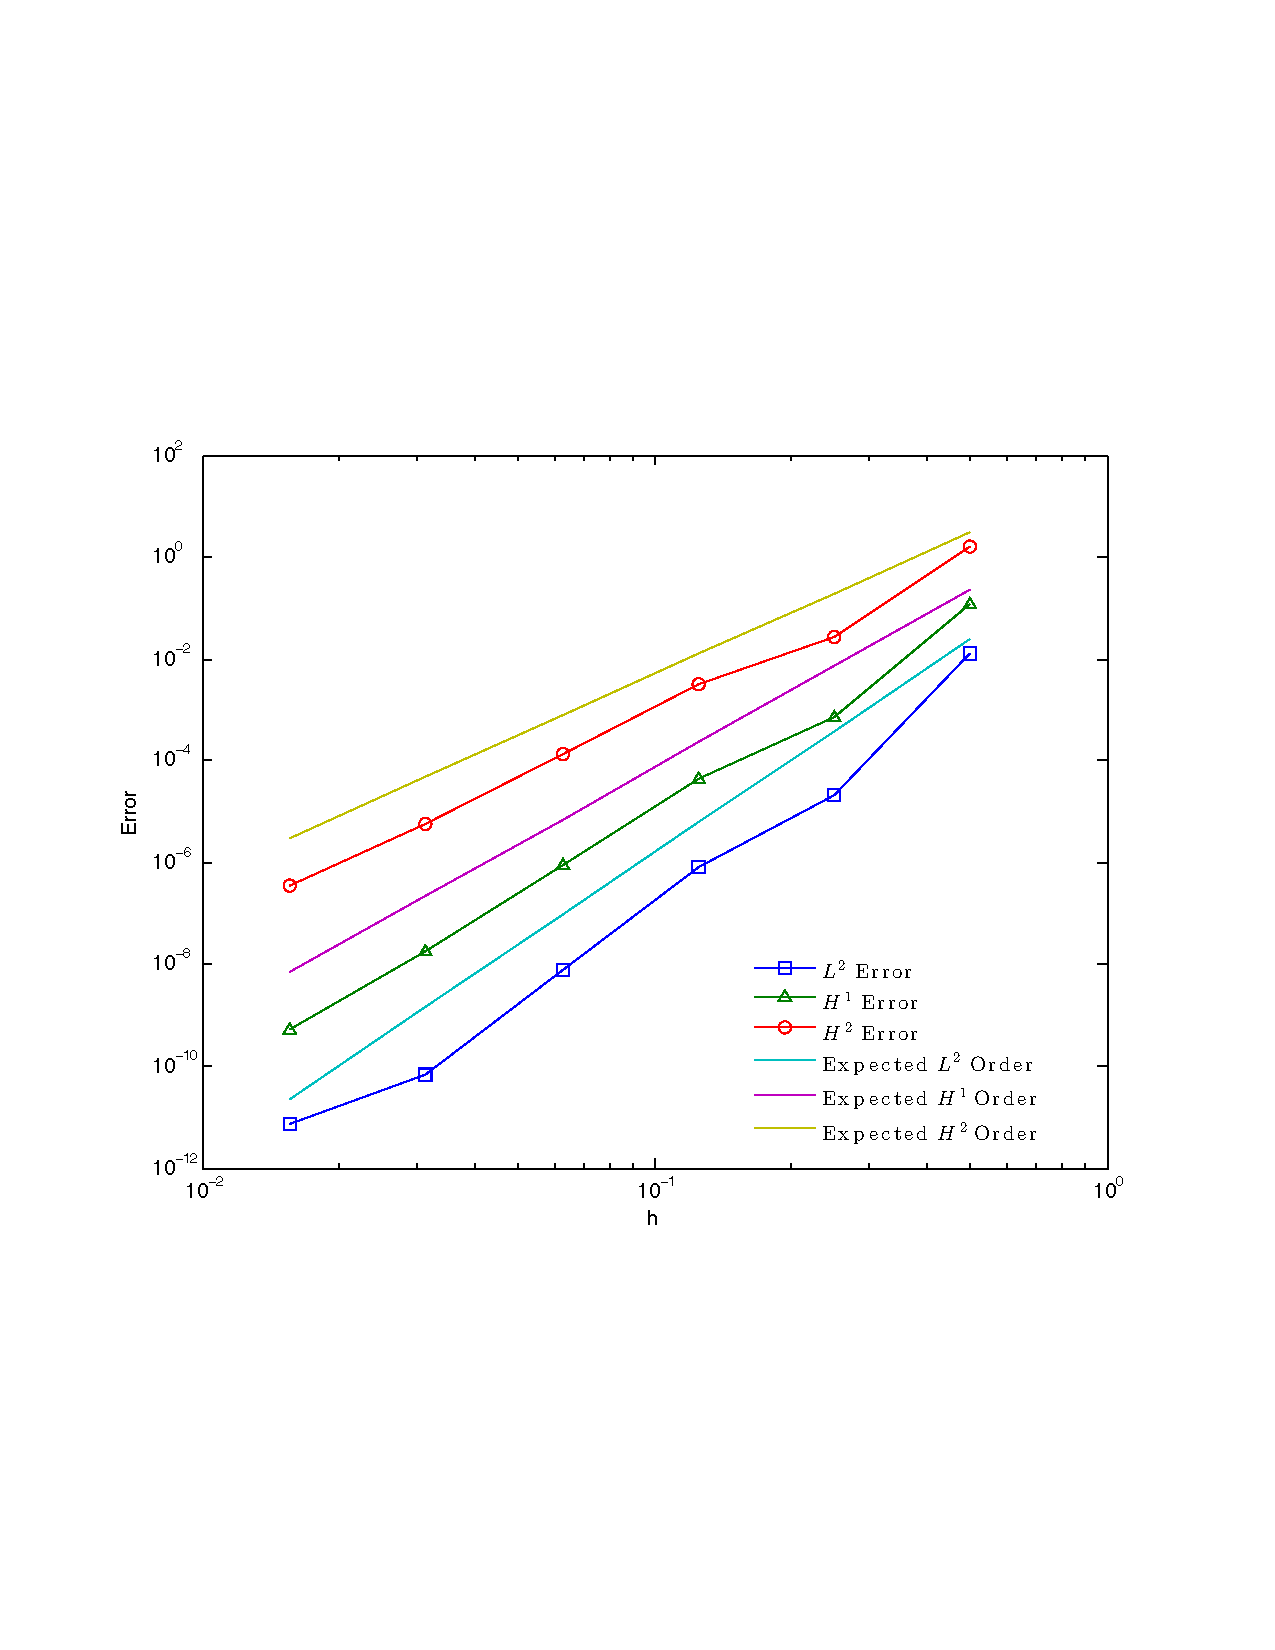
\includegraphics[scale=0.6]{sin2sin2sinSpaceConvergence.pdf}
    \caption{Observed orders of convergence in space for Argyris applied to
      \eqref{eqn:QGE_psi} with the exact solution \eqref{eqn:Test1} using
      implicit Euler for the time discretization.}
  \label{fig:Test1Space}
  \end{center}
\end{figure}

\subsubsection*{Test 2}
For this test we take the exact solution to be
\begin{equation}
  \psi(t;x,y) = \left[(1-x)\left(1-e^{-0.1\,x\,t}\right) \sin \pi y\right]^2
  \label{eqn:Test2}
\end{equation}
which is very similar to \textbf{Test 4} in \cite{Foster}. Here we add the time
dependence in the exponential term and let $\Omega = [0,1]^2$. The time interval
for integration is $t = [0,1]$. This test will have an intensifying western
boundary layer as time increases.
\begin{table}
\begin{center}
  \begin{tabular}{|c|c|c|c|c|}
    \hline
    $k$ & $h$ & DoFs & $e_{L^2}$ & $L^2$ order \\% & $e_{H^1}$ & $H^1$ order & $e_{H^2}$ &         $H^2$ order \\
    \hline
$\nicefrac{1}{8}$ & $\nicefrac{1}{20}$ & $1158$ & $5.00\times 10^{-7}$ & $-$ \\% & $2.576\times 10^{-6}$ & $-$ & $1.738\times 10^{-5}$ & $-$ \\
$\nicefrac{1}{16}$ & $\nicefrac{1}{20}$ & $1158$ & $2.49\times 10^{-7}$ & $1.01$ \\% & $1.284\times 10^{-6}$ & $1.005$ & $8.691\times 10^{-6}$ & $1$ \\
$\nicefrac{1}{32}$ & $\nicefrac{1}{20}$ & $1158$ & $1.24\times 10^{-7}$ & $1.00$ \\% & $6.409\times 10^{-7}$ & $1.002$ & $4.392\times 10^{-6}$ & $0.9846$ \\
$\nicefrac{1}{64}$ & $\nicefrac{1}{20}$ & $1158$ & $6.21\times 10^{-8}$ & $1.00$ \\% & $3.203\times 10^{-7}$ & $1.001$ & $2.299\times 10^{-6}$ & $0.9342$ \\
$\nicefrac{1}{128}$ & $\nicefrac{1}{20}$ & $1158$ & $3.11\times 10^{-8}$ & $1.00$ \\% & $1.602\times 10^{-7}$ & $0.9995$ & $1.337\times 10^{-6}$ & $0.7817$ \\
$\nicefrac{1}{256}$ & $\nicefrac{1}{20}$ & $1158$ & $1.55\times 10^{-8}$ & $1.00$ \\% & $8.034\times 10^{-8}$ & $0.9957$ & $9.564\times 10^{-7}$ & $0.4834$ \\
$\nicefrac{1}{512}$ & $\nicefrac{1}{20}$ & $1158$ & $7.76\times 10^{-9}$ & $1.00$ \\% & $4.068\times 10^{-8}$ & $0.9818$ & $8.346\times 10^{-7}$ & $0.1966$ \\
    \hline
  \end{tabular}
\end{center}
  \caption{Observed order of convergence for Implicit-Euler applied to
    \eqref{eqn:QGE_psi} with the exact solution \eqref{eqn:Test2}. Note the observed
    order of convergence matches the theoretical error estimates developed in
    \autoref{sec:QGEError}.}
  \label{tab:Test2Time}
\end{table}

\subsection{North Atlantic}
The North Atlantic Ocean is intensely studied and therefore makes a good test
problem for evaluating the performance of our model \cite{Myers}. Hence, we have
created a FE mesh of the North Atlantic which extend from $15^\circ N$ to $65^\circ
N$ using GMSH \cite{GMSH}. The coastline data was obtain from GSHHS \cite{GSHHS}.
The finite element spacing was specified to be {\color{red} $15km$}.  Major
islands such as Cuba, Hispaniola Greenland, Great Britain, and Ireland were
connected to the nearest continent and hard boundaries were created at the
northern and southern most extents of the North Atlantic. The resultant FE mesh
can be seen in \autoref{fig:AtlanticMesh}.

\begin{figure}
  \begin{center}
    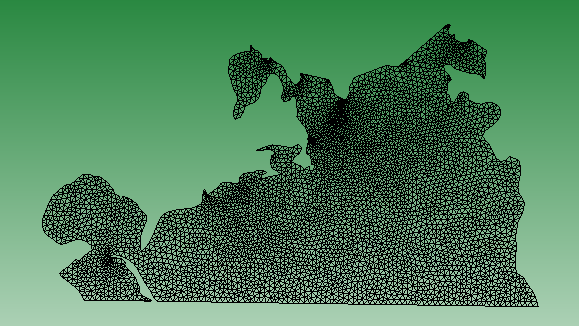
\includegraphics[scale=0.5]{NAMesh.png}
    \caption{Mesh of the North Atlantic created using GMSH \cite{GMSH}.}
    \label{fig:AtlanticMesh}
  \end{center}
\end{figure}

The experiment used annual mean wind forcing obtained from Hellerman and
Rosenstein (1983). We choose similar similar parameters as those used in
\cite{delSastre04} and are summarized in \autoref{tab:AtlanticParameters}.

\begin{table}
  \begin{center}
  \begin{tabular}{|l|l|}
    \hline
    $A$ & $2000m^2s^{-1}$\\
    \hline
    $\theta_0$ & $40^\circ$ \\
    \hline
    $\omega$ & $7.2526\times 10^{-5}s^{-1}$ \\
    \hline
    $H$ & $1000m$ \\
    \hline
    $L$ & $1000km$ \\
    \hline
    $r_e$ & $6378.1km$ \\
    \hline
    $\rho$ & $1027 \nicefrac{kg}{m^3}$ \\
    \hline
  \end{tabular}
  \end{center}
  \caption{Table of parameter values used for the simulations of the North
    Atlantic. \cite{delSastre04}}
  \label{tab:AtlanticParameters}
\end{table}

Using the relation
\begin{equation}
  \beta = \frac{2\omega}{r_e}\cos \theta_0
  \label{eqn:Beta}
\end{equation}
and the parameters given in \autoref{tab:AtlanticParameters} we see that
\begin{equation*}
  \beta \approx 1.742\times 10^{-11}\, m^{-1}\,s^{-1}.
\end{equation*}
Using this approximation for $\beta$ and \eqref{eqn:velocity_scale} with
{\color{red}$\tau_0 = 0.6\, dyne\, cm^{-2}$ \cite{Hellerman} gives the following
approximation for the characteristic velocity
\begin{equation*}
%  \begin{split}
%    U &= \frac{3.1415 \cdot 0.6 dyne\, cm^{-2}}{1027 \nicefrac{kg}{m^3} \cdot
%      1000\, m \cdot 1.742 \times 10^{-11}\,m^{-1}\,s^{-1} \cdot 1000\, km} \\
    U = 1.054\times 10^{-2} \nicefrac{m}{s}.
%  \end{split}
\end{equation*}
Therefore, the Rossby number is
\begin{equation*}
%  Ro = \frac{1.054\times 10^{-2} \nicefrac{m}{s}}{1.742\times 10^{-11} m^{-1}
%    s^{-1} (1000 km)^2}
  Ro = 6.051\times 10^{-4}
\end{equation*}
and the Reynolds number is
\begin{equation*}
  Re = 5.27.
\end{equation*}}

From the length scale $L$ and the velocity scale $U$ we see that the time scale
is approximately $T = 3\, years$. Thus, a nondimensional time interval of
$[0,120]$, which was also used by Bermejo et al \cite{delSastre04}, corresponds
to a total of $360$ years. We use the same dimensional time step used in
\cite{delSastre04}, which was $\Delta t = 2\, hours$. This time step corresponds
to nondimensional time step of $k = 7.6053 \times 10^{-5}$. {\color{red} This
may be unrealistic.}

\subsection{Mediterranean}

\begin{figure}
  \begin{center}
    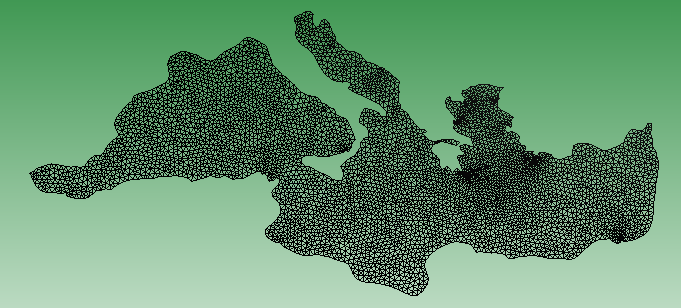
\includegraphics[scale=0.5]{MedMesh.png}
    \caption{Mesh of the Mediterranean created using GMSH \cite{GMSH}.}
    \label{fig:MedMesh}
  \end{center}
\end{figure}

